\documentclass[11pt, twoside]{report}
\usepackage[utf8]{inputenc}
\usepackage{graphicx}
\usepackage{wrapfig}
\usepackage[a4paper, width=150mm, top=25mm, bottom=30mm, bindingoffset=20mm]{geometry}
\usepackage[toc,page]{appendix}
\usepackage{pdfpages}
\usepackage{natbib}
\usepackage{pdflscape}
\usepackage{longtable}
\usepackage{tikz}
\usepackage{multirow}
\usepackage{textcomp}
\usepackage{fancyhdr}
\usepackage{helvet}
\usepackage{hyphenat}
\usepackage{listings}
\usepackage{color}	
\usepackage[hidelinks]{hyperref}
\usepackage{pgfplots}
\renewcommand{\familydefault}{\sfdefault}
\def\checkmark{\tikz\fill[scale=0.4](0,.35) -- (.25,0) -- (1,.7) -- (.25,.15) -- cycle;} 
\pagestyle{fancy}
\fancyhf{}
\fancyhead[LE, RO]{\thepage}
\fancyhead[LO, RE]{\leftmark}
\fancyfoot[c]{Bournemouth University, Department of Computing and Informatics, Final Year Project}
\setlength{\headheight}{13.6pt}
\linespread{1.3}
\bibliographystyle{buHarvard}
\bibpunct{(}{)}{,}{a}{}{ }
\graphicspath{ {images/}{appendices/} }
\footskip = 15mm
\definecolor{mygreen}{rgb}{0,0.6,0}
\definecolor{mygray}{rgb}{0.5,0.5,0.5}
\definecolor{mymauve}{rgb}{0.58,0,0.82}
\pgfplotsset{compat=1.13}

\lstset{ %
  backgroundcolor=\color{white},   % choose the background color; you must add \usepackage{color} or \usepackage{xcolor}
  basicstyle=\ttfamily\footnotesize,        % the size of the fonts that are used for the code
  breakatwhitespace=false,         % sets if automatic breaks should only happen at whitespace
  breaklines=true,                 % sets automatic line breaking
  captionpos=b,                    % sets the caption-position to bottom
  commentstyle=\color{mygreen},    % comment style
  escapeinside={\%*}{*)},          % if you want to add LaTeX within your code
  extendedchars=true,              % lets you use non-ASCII characters; for 8-bits encodings only, does not work with UTF-8
  keepspaces=true,                 % keeps spaces in text, useful for keeping indentation of code (possibly needs columns=flexible)
  keywordstyle=\color{blue},       % keyword style
  otherkeywords={*,...},           % if you want to add more keywords to the set
  numbers=left,                    % where to put the line-numbers; possible values are (none, left, right)
  numbersep=5pt,                   % how far the line-numbers are from the code
  numberstyle=\tiny\color{mygray}, % the style that is used for the line-numbers
  rulecolor=\color{black},         % if not set, the frame-color may be changed on line-breaks within not-black text (e.g. comments (green here))
  showspaces=false,                % show spaces everywhere adding particular underscores; it overrides 'showstringspaces'
  showstringspaces=false,          % underline spaces within strings only
  showtabs=false,                  % show tabs within strings adding particular underscores
  stepnumber=1,                    % the step between two line-numbers. If it's 1, each line will be numbered
  stringstyle=\color{mymauve},     % string literal style
  tabsize=2,	                   % sets default tabsize to 2 spaces
}


\begin{document}
\pagenumbering{Alph}

%TC:ignore


\includepdf{cover.pdf}
\pagenumbering{roman}

\vspace*{\fill}
\begingroup
\centering
Faculty of Science \& Technology

Department of Computing and Informatics

Final Year Project

\endgroup
\vspace*{\fill}

\chapter*{Abstract}
Lorem ipsum dolor sit amet, consectetur adipisicing elit, sed do eiusmod tempor incididunt ut labore et dolore magna aliqua. 
Ut enim ad minim veniam, quis nostrud exercitation ullamco laboris nisi ut aliquip ex ea commodo consequat. 
Duis aute irure dolor in reprehenderit in voluptate velit esse cillum dolore eu fugiat nulla pariatur. 
Excepteur sint occaecat cupidatat non proident, sunt in culpa qui officia deserunt mollit anim id est laborum.

%!TEX root = ../main.tex
\chapter*{Dissertation Declaration}
{\linespread{1.0} %The BU template dictates this to be this line spacing
I agree that, should the University wish to retain it for reference purposes, a copy of my dissertation may be held by Bournemouth University normally for a period of 3 academic years. I understand that once the retention period has expired my dissertation will be destroyed.

\section*{Confidentiality}
I confirm that this dissertation does not contain information of a commercial or confidential nature or include personal information other than that which would normally be in the public domain unless the relevant permissions have been obtained. In particular any information which identifies a particular individual's religious or political beliefs, information relating to their health, ethnicity, criminal history or sex life has been anonymised unless permission has been granted for its publication from the person to whom it relates.

\section*{Copyright}
The copyright for this dissertation remains with me.
 
\section*{Requests for Information}
I agree that this dissertation may be made available as the result of a request for information under the Freedom of Information Act.
\\ \newline
\textbf{Signed:}
\\
Name: Michael Porter
\\
Date:
\\
Programme: BSc Software Engineering
}

\chapter*{Original Work Declaration}

This dissertation and the project that it is based on are my own work, except where stated, in accordance with University regulations.
\\ \newline
\textbf{Signed:}

%!TEX root = ../main.tex
\chapter*{Acknowledgements}
These are my acknowledgements

%Lys
%Damien
%Jake
%The good people of StackOverflow

\hypersetup{
	citecolor=black,
	filecolor=black,
	linkcolor=black,
	urlcolor=black
}

\tableofcontents
\listoffigures

\cleardoublepage
\pagenumbering{arabic}

%TC:endignore

%1000 words
%!TEX root = ../main.tex
\chapter{Introduction}
\label{chap:intro}

\section{Problem Definition}
Parents can often find it difficult to motivate their children to perform chores in a timely manner. 
Many parents have attempted to implement a simple reward system to incentivise their children, but often fail to keep up with the rewards or maintain the tracking needed to make the positive reinforcement truly effective.
I believe this is a problem that all parents face, and one we have all faced as children ourselves.  

\section{Proposed Artefact}
I want to create a proof-of-concept mobile application that will allow parents to assign tasks and rewards to their children in the form of `quests' in a role-playing game, effectively gamifying chores. 
The quests can take the form of ``Tidy your room'' or ``Complete your homework'' and offer rewards of experience points (XP) and gold. The application will also allow the child to create an in-game character that they can customise and level up using aforementioned gold and XP.
I believe the app will provide children with incentive and positive reinforcement to achieve more.

\section{Clients}
The key clients for this app will be the parent(s) or guardians inputting quests into the game and marking a quest as complete once they have inspected the work. 
The child will also be able to view quests, notify the parents that a quest requirement is ready for inspection, and purchase real life rewards from a reward shop.
Parents will also be able to monitor their children's activities and progress, whilst approving or rejecting various activities that the child may encounter whilst using the application. 

\section{Aims and Objectives}
The aim of this project is to evaluate the usefulness of game-based rewards for children performing chores. 
To achieve this, I have identified the following objectives for the software artefact:

\begin{itemize}
	\item Create a well designed mobile application, capable of tracking progress and offering rewards for chores and adhering to the Android Developer specifications
	\item Create a secure and robust public API to allow applications to connect to the the artefact's service
	\item Utilize appropriate technologies to securely create the two deliverables to a high quality
	\item Utilize test-driven development to provide automated testing, ensuring test coverage of over 80\% for the API
\end{itemize}

\section{Risks}
In this project, I will be working with a variety of technologies that I have not previously used or am not very experienced with, such as Flask, Android and REST. 
This presents a likely risk that the learning curves of these tools may be steeper than expected.
If this occurs, it is likely that initial time-frame estimates for the development will be inaccurate, as features involving these technologies may incur delays.
The scale and importance of the above delays could, in themselves, lead to the project not entirely fulfilling the above objectives. I believe this makes the above risk high severity.
In order to mitigate this, I have researched a variety of different learning materials that I will be able to access throughout the project to help me better understand these tools.
Furthermore, I have sourced potential help from my placement company, where colleagues have agreed to provide guidance in areas they are experienced in.

As this is a task management app, the artefact risks becoming more of a hindrance then a help.
There is a possibility that the app could become too intrusive to parents giving their children a task, as what would normally be a simple request could be delayed by the additional process of entering and tracking the task.
If this was to occur, it would result in the app being less desirable to use.
However, I believe that if I put a sufficient focus on usability within the app and attempt to design my use cases to have as little resistance as possible, I can avoid this risk.
I can also mitigate this risk by offering Parent users their own version of the app, which would allow them to circumvent any security features designed to stop a Child from giving themselves rewards.

%2000 words
%!TEX root = ../main.tex

\chapter{Background Study}
\label{chap:litReview}
This is the background study part


%1500 words
%!TEX root = ../main.tex
\chapter{Requirements and Analysis}
\label{chap:methodology}

\section{Defining Requirements}
\subsection{Functional Requirements}
Functional requirements are, in simple terms, things that the system should be able to do. 
Generally, functional requirements will specify behaviours, common goals, or functionality that one may require from the software being designed.
Typical examples of these could include `display customer' or `add order'. 
The overall quality of the software can be evaluated by the quality and effectiveness of these individual features.

\subsection{Non-functional Requirements}
Non-functional requirements are defined as ``Software requirements that describes not what the software will do, but how the software will do it'' \citep[p.6]{chung2012non}.
This includes examples such as the software's performance requirements, usability, quality of services, reliability etc.
These are generally more subjective aspects of the software requirements and are therefore harder to evaluate. 
It is important, however, that they still be considered during development iterations.

Software specifications are made up of both functional and non-functional requirements \citep{chung2012non}. 

\section{Gathering Requirements}
\subsection{Actors}
When determining use cases, the first step is to define the actors in the software.
In UML, an actor is defined as a ``a type of role played by an entity that interacts with the subject (e.g., by exchanging signals and data), but which is external to the subject.'' \citep[p.586]{omg2007unified}.
Actors may represent human users of the system or other external systems that will interact with the software being modelled.
Different actors will have different objectives for using the application and it is important that the requirements of each actor are analysed to ensure the application is suitable. 
In this project there are two key actors, the Child and the Parent. 
The Child marks quests as complete and creates an character. In actual usage, this will usually be a dependent of the primary user. 
The Parent assigns, manages, and approves their child's quests. In actual usage, this will usually be a real-life parent or guardian of the secondary user.

\subsection{Identifying Features}
A useful first step in identifying the features of the software artefact is to use brainstorming to quickly list features that could be possible for the application, without regard to the suitability or feasibility of the ideas.
Essentially, the goal of brainstorming is to achieve quantity over quality \citep[p.144]{leffingwell2000managing}.
Once a wide breadth of ideas has been listed out on a brainstorm, it is recommended to begin an `idea reduction' stage, where ideas are briefly evaluated to rule out obviously infeasible ideas to obtain a solid list of features that can be more deeply evaluated at a later stage.
The process for brainstorming the application involved looking at the features of similar existing apps - such as task management apps or apps gamified for children - whilst keeping in mind the original objectives of this project.
The results of this brainstorming process can be seen in figure \ref{fig:brainstorm}.

\begin{figure}[ht]
	\centering
	\includegraphics[scale=0.55]{images/Brainstorm.png}
	\caption{Brainstorm of Potential Features}
	\label{fig:brainstorm}
\end{figure} 
% TODO: standardise capitalisation within the figure? Level/apps/collecting etc.
%Still has the name KidQuest in this too  
%Colour coordinate

\subsection{MoSCoW}
Developing a software project is a complicated procedure with many potential roadblocks to be faced.
As identified in my risk analysis, there are several risks that can cause significant delays to the project, which in turn could be disastrous to the project due to its fixed deadline.
Research by \cite{requirementsprioritization} has shown that only 16\% of all software projects are delivered on time and within budget, which has harrowing implications for the schedule of the project.

In light of this, a useful next step is to prioritise the tasks ahead by determining which features are most vital to the project and will, therefore, require most time and urgency.
MoSCoW is an easy method of dividing requirements into a clear hierarchy of four categories that establish a priority for the features or requirements of a software project \citep[p.517]{hatton2008choosing}.
This MoSCoW list will serve as the final list of features that I hope to include within this project and will be referred to as my `to-do list' throughout development. 
It is important to explicitly note, however, that this is not a target of features that will be in the application, but rather a hierarchical `wish list' of features that may or may not be achieved, depending on how development progresses within the time frame.
I have separated the functional requirements (FRxx) and non-functional requirements (NRxx) into the four MoSCoW categories in the following list:

\subsubsection{Must Have}
There are some features that will be vital to the success of the project and can cause delays to the release of the software if they are not finished on time.
These should be the first features developed in the software and be thoroughly tested to ensure high quality.

\begin{center}
\fontsize{8}{10}\selectfont
\begin{longtable}{|C{1cm}|L{3cm}|L{8cm}|}
	\hline
	\textbf{No.} & \multicolumn{1}{C{3cm}}{\textbf{Feature}} & \multicolumn{1}{|C{8cm}|}{\textbf{Description}} \\ \hline
	FR01 & Child Tasks App & A Child can login and see tasks to complete, and mark as completed accordingly \\ \hline
	FR02 & Parent Control App & A Parent can login and view details about the Child's account \\ \hline
	FR03 & RPG Rewards & Child users will be rewarded with experience points and will level up after obtaining certain amounts \\ \hline
	FR04 & Gold Rewards & Child users will be given a gold reward for completing tasks on time \\ \hline
	FR05 & Reward shop & Parents will be able to set real life rewards for the Child to purchase using earned gold \\ \hline
	FR06 & REST API back-end & Implement a REST API server that the Parent and Child apps can use to communicate with each other, instead of phone to phone communication \\ \hline
	NR01 & Reliability & App must not crash, and must handle errors gracefully \\ \hline
	NR02 & Security & Server must not make user information accessible without correct authentication \\ \hline
\end{longtable}
\end{center}

\subsubsection{Should Have}
These are features that are important to have, but are not integral to the app's main functionality, so will not render the app useless if they are incomplete at the end of the process.

\begin{center}
\fontsize{8}{10}\selectfont
\begin{longtable}{|C{1cm}|L{3cm}|L{8cm}|}
	\hline
	\textbf{No.} & \multicolumn{1}{C{3cm}}{\textbf{Feature}} & \multicolumn{1}{|C{8cm}|}{\textbf{Description}} \\ \hline
	FR07 & Preset Quests & Allow Parent uers to choose from a list of preset tasks generated by the server, such as trending tasks \\ \hline
	FR08 & Friends List & Allow Child users to add each other as friends in the app. The adding of friends should be monitored and approved by Parent users \\ \hline
	FR09 & Notifications & Alert a user whenever their respective Parent/Child performs certain actions \\ \hline
	NR03 & Portability & The server should be platform agnostic and serve content regardless of client device \\ \hline
	NR04 & Usability & User must be able to easily navigate between various screens \\ \hline
	NR05 & Usability & The app should be responsive and reliable \\ \hline 
	NR06 & Android Developer Guidelines & App must make a best effort to follow the Android Developer Material guidelines laid out by Google \\ \hline
\end{longtable}
\end{center}

\subsubsection{Could Have}
This describes features that would be preferable to have in the project and could be looked at, if there is time to, at the end of the project.
However, it is important to be wary of scope creep and recognise that any feature added will not only add development time, but testing and documentation time too.

\begin{center}
\fontsize{8}{10}\selectfont
\begin{longtable}{|C{1cm}|L{3cm}|L{8cm}|}
	\hline
	\textbf{No.} & \multicolumn{1}{C{3cm}}{\textbf{Feature}} & \multicolumn{1}{|C{8cm}|}{\textbf{Description}} \\ \hline
	FR10 & Friend Battles & Child users can select friends to `battle' with and compete with \\ \hline
	FR11 & Graph Friend Selection & Graph selection UI for inviting friends to undertake group quests \\ \hline
	FR12 & Web application & Allow Parent/Child to use a web application to access their accounts \\ \hline
\end{longtable}
\end{center}

\subsubsection{Won't Have}
Suggested features that are not feasible for this release, due to time and resource constraints.
These could potentially be re-raised for a future update to the software.

\begin{center}
\fontsize{8}{10}\selectfont
\begin{longtable}{|C{1cm}|L{3cm}|L{8cm}|}
	\hline
	\textbf{No.} & \multicolumn{1}{C{3cm}}{\textbf{Feature}} & \multicolumn{1}{|C{8cm}|}{\textbf{Description}} \\ \hline
	FR13 & Sound Effects & Music and audio effects when certain events are completed \\ \hline
	FR14 & Character Graphics & Artistically designed graphical interface \\ \hline
	FR15 & Leaderboards & A constantly updated ranking of calculated `scores' between befriended users \\ \hline
\end{longtable}
\end{center}

\subsection{Use Case Diagrams}
In order to properly specify the requirements for a user in more detail, it is useful to plan out the various use cases a user may take in a use case diagram.  
The purpose of a use case diagram is to show the actors the system, their goals, and how those goals work in relation to each other.
Use case diagrams are also helpful to visualise an outside view of a system and gather requirements - although in this case I am using the diagram to refine the requirements that I have already mapped out.

\begin{figure}[ht]
	\centering
	\includegraphics[scale=0.55]{images/UseCaseDiagram.png}
	\caption{Use case diagram of the `Must Have' functional requirements}
	\label{fig:usecasediagram}
\end{figure} 
% again - check your capitalisation.
In figure \ref{fig:usecasediagram}, you can see the two actors in the system and the relationships between the tasks that they may take. 
The diagram also lists tasks that are extended from another task such as `view pending task', which, for all intents and purposes, is the same feature as `view tasks'. The difference is that you only see a subset of the tasks. 
You can also more clearly see the layout of the reward shop, where the use case details how the Parent can view the shop to add or remove rewards, whereas the Child can view the shop to purchase rewards.

%1500 words
%!TEX root = ../main.tex

% 1000-2000 words

\chapter{Design}

\section{Development Methodologies}

\subsection{Waterfall}
The waterfall design methodology is a sequential design processed focused on the project progressing to each stage of development one at a time, for example, the design stage of the software would not take place until all requirements have been gathered and finalised.
Waterfall is considered to be a very structured methodology and is particularly useful when the requirements are well known and are fixed before the project begins and when the project and the technologies are well understood.

However, due to the rigidity of the Waterfall method, particularly around the planning phase, it is easy for mistakes made early on in the software development life cycle to become embedded within the project and be carried forward to later stages. CITATION NEEDED
For example, if a mistake is made during the requirements gathering phase and is not noticed until a later phase of the project, it will be very costly to change.

\subsection{Agile}
The Agile design methodology is a well established and iterative design process that involves regularly moving between the stages of the project in a non-sequential manner. 

One of the key principles of agile development is regular and iterative testing throughout the software development life cycle.
As I am a single developer working on this project, this is beneficial to me as it helps give early sight of potential design issues early in the project.

Agile is also very adaptable.
It allows for more flexibility to the software when design issues undoubtedly arise by not setting the specification for the whole project in stone too early.
By iteratively planning the design of the project, it allows for quick responses to feedback and if one part of the project is changed, it should have minimal effect on the rest of the project stages. 

The agile methodology also extends to the testing of the project.
By iteratively testing the software at various stages in the life cycle, it gives more chances to catch bugs early.
Under agile, defects discovered in software should be fixed as soon as possible after discovery \citep{beck2001agile}.

In a study by \cite{talby2006}, it was found that by following this practice, defects took less time to fix than without.
This may be due to the fact that the developed features are still fresh in the mind of the developer, and is therefore more easily able to see the problem area and fix.
The study also found that by keeping the bugs fixed and the code base stable throughout the project, it actually made the development phases of the project faster.
Furthermore, agile testing helps minimize the risks of bugs making it into the final artefact. 
If I were to have a single testing phase at the end of the project, it is possible that there would be more bugs than I had anticipated and that I would run out of time to properly fix them all. 
By using agile testing, this risk is minimized by allowing me to better manage the time of testing, as I will be able to delay or cancel the development of certain low priority features earlier in the project to allow me time to ensure a quality project.

\section{Development Processes}
There are also many sub-processes that are born out of or tie into Agile which could be beneficial for my project.

\subsection{Feature-Driven Development}
Feature-driven development (FDD) is an lightweight and iterative software development process which involves mapping out the feature list of the software as the `plan' for it's development.


\subsection{Test-Driven Development}
A key factor of test-driven development is planning out the testing phases of the project before the development of that phase begins.
The key workflow of TDD is as follows \citep{Beck:2002:TDD:579193}
\begin{enumerate}
	\item Add a test that tests the new feature works.
	\item Run all tests and see the new one fail.
	\item Write the code that makes the test pass.
	\item Run all tests and see them all succeed.
	\item Refactor the code and tests to remove duplication.
	\item Repeat.
\end{enumerate}

Under this process, a feature is complete when the tests show that it works.

A study by \cite{George:2003:IIT:952532.952753} developers following TDD produced higher quality code which passed 18\% more functional tests.



\subsection{Behaviour-Driven Development}



After planning out the requirements, the next step in the design of KidQuest was to plan out the database structure.
I created an entity relationship to map out the various tables needed and the relationships between them.

\begin{figure}[t]
	\centering
	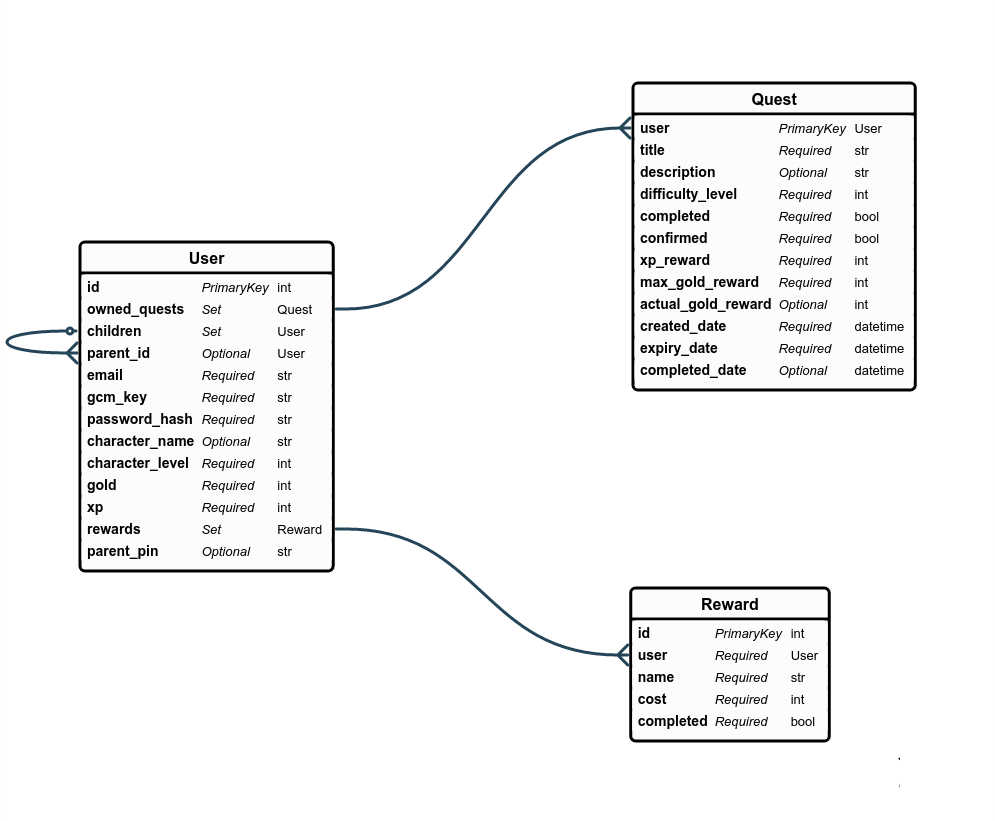
\includegraphics[width=0.75\textwidth]{images/entityRelationshipDiagram.png}
	\caption{Entity-Relationship Diagram}
	\label{fig:ERD}
\end{figure}

I have chosen to create the application in the Android SDK largely due to my previous experience with Java and Android. 
Furthermore, I believe Android is more applicable to the target audience of the app, as Android owns 82.8\% of the smartphone market share as of 2015.
%http://www.idc.com/prodserv/smartphone-os-market-share.jsp
I believe that parents are also more likely to buy their children Android phones than other brands due to the lower price point, making them more appealing when considering the likelihood of them being lost or broken by a child.

For the data analytics, I have opted to use web services written in Flask microframework for python, hosted on a server running Ubuntu Server 14.04. 
I have chosen python due to it's strong backing and community support in data analytics, and is one of the main languages of choice for scientists and statisticians.
The flask framework was chosen specifically as it is very simple to write and host RESTful APIs over the web.

To safely store and version control the code, I used a GitHub private repository to host my code in cloud storage and allow for me to better manage changes to the code-base. 

\section{Aesthetic Design}

\subsection{Wireframes}

\subsection{Android Developer Guidelines}

\section{Usability}

\section{Use Cases}	

\section{Development Style}


%3000 words
%!TEX root = ../main.tex
\chapter{Implementation and Evaluation}

For clarity, I present the implementation and evaluation together and split the presentation by the natural split in the code which is the server and application.

\section{Server}
\subsection{Representational State Transfer (REST)}
To structure the server's web services, I have chosen to use a REST architecture style.
REST involves dividing the web services into specific objects which can be accessed through sending a request to that object's URL. 
This is called an `endpoint' or a `URI'.
These endpoints are then connected to via different HTTP methods, such as the following:
\begin{description}[align=left]
	\item [GET] Retrieves an item or list of items.
	\item [POST] Creates a new item.
	\item [PUT] Updates an existing item or list of items.
	\item [DELETE] Deletes an item. 
\end{description}
For example, if someone wanted to retrieve all users of a REST service, they could send a GET request to the `/users/' endpoint. 
If, however, they wanted to retrieve a specific user, they would send a GET request to `/users/$x$/' where $x$ is the user's ID.
And finally, sending a POST request to `/users/$x$/quests/' would create a a new quest for user $x$.

Collectively, these request methods and endpoints will form the basis for all communication with the server. 
A full plan for the endpoints of the server artefact can be seen in appendix \ref{appendix:endpoints} and examples of requests in \ref{appendix:requests}.

\subsubsection{JSON}
In order to facilitate communication between the server and devices, JSON has been chosen as the primary messaging format for this system.
JSON is a format of transmitting data in a both human and machine readable way using key value pairs.
When the server is required to return objects from the database, it will be able to serialise the python object into JSON text and return it in the request.
The application will then be able to de-serialise the JSON back into a Java object, translating the JSON values back into object properties.
Examples of possible requests can be seen in appendix \ref{appendix:requests}.

\subsection{Flask}
For the server-side implementation, I will need tools that allow me to easily create a web service API and provide controlled access to functionality over the web.
For this task, I chose to use Flask as it is well established within the Python community and is relatively easy to set up and maintain. 
Flask is suitable for both quick prototyping of web-services and reliable deployment/hosting of the functionality over the internet.

By utilising Flask, I was able to easily translate a user's web request into a method call, with relevant parameters, using the following code:
\lstinputlisting[language=python]{codesnippets/getrewards.py}
This short code snippet shows the method used to return all rewards in the reward shop for a user.
This method is activated upon sending a GET request to the endpoint such as `server\_host\_name:5000/api/user/1/rewards/', and will return the rewards for the first user in JSON format, provided the attached authentication details match that user. 

\subsection{Database}
\subsubsection{Object-Relational Mapper}
I chose to use a pre-built Object Relational Mapping (ORM) library to interface with the database, rather than crafting particular queries on an ad hoc basis. 
%Feel like I need another way to say this line
This was primarily for more ease-of-use purposes than any performance reasons. 
I decided upon using SQLAlchemy as the ORM for the server due to strong Flask support.
Specifically, the Flask-SQLAlchemy library was utilised to provide Flask specific functions that could be used to interface with the database.
Implementing an ORM also allows me to more easily protect the application against SQL injection, as Flask purposefully escapes special characters that would allow such an attack \citep[p.15]{copeland2008essential}.

\subsubsection{SQLite}
I have opted to use SQLite to store the user data in the server.
SQLite is a very lightweight RDBMS that is well supported by the Flask-SQLAlchemy library.
The database tables will be automatically generated out of the classes created in Flask on the first run of an application, as well the relationships described in figure \ref{fig:erd}. 

\subsection{Evaluation}
Of my objectives, there are two that are relevant to the server:
1. Create a secure and robust public API to allow applications to connect to the artefact's service.
The server application successfully provides a public API that provides web services to connecting clients.
The server provides the necessary information for clients securely, by requiring successful HTTP authentication to retrieve information about an user or any of it's quests/rewards.
The server is resilient to crashes and automatically rejects bad requests before the invalid data can be stored in the database, and
2. Utilise test-driven development to provide automated testing, ensuring test coverage of over 80\% for the API
Using the practice of test-driven development for the server API was a general success. 
For some parts, the methodology was found to be rather strict and caused some delays to development time.
However, once the practice had been used for a little while, it began to drastically improve development time, particularly in the case of debugging that arose during development.
Furthermore, during testing phases, the tested code passed many of its functional tests on the first try, which is likely due to the fact that it is regularly tested during the development process.
Overall, it was found that most features took slightly longer to develop, but took significantly less time during testing phases.
These findings agree with the research in chapter 2, as \cite{IBMTDD} found similar results of reduced productivity, but it resulted in code with less defects.

The final result for automated test coverage came in at 91\% code coverage for the server, exceeding the 80\% target, and analysis of the code shows all major server functions were covered by automated unit tests.

\section{Application}
\subsection{Android}
Android has been chosen for this application due to the large success and market hold of the operating system.
Primarily I will be aiming to support Android versions down to API level 16 (Jelly Bean 4.1) \footnotemark[1].
This decision has been made as appendix \ref{appendix:sdkmarketshare} shows that by supporting this far back, the application will be compatible with over 95\% of current phones. 
Older versions than this will not be targeted, as development and testing time is limited and it would mean that many features would have to be limited due to lacking functionality within these older versions.

\footnotetext[1]{Many features included in recent Android versions will not work in older versions. Android development allows you to specify a minimum Android version to prevent the use of features that will not work on older phones.}

\subsection{Google Cloud Messaging}
The app will be responsible for relaying information between the parent and child clients in a reliable and timely manner.
In Android, this can be achieved using push notifications relayed through the Google Cloud Messaging (GCM) service.
GCM can be utilised to send messages to an Android device, but is largely unreliable \citep{gcmreliability} and therefore should only be used for notifications, rather than the transmission of data.
The service requires that the server registers with the GCM to retrieve an API key and that the user device registers to retrieve a GCM registration ID \citep{gcm}. 
When a user registers with the artefact server, the registration ID is stored wtihin the database to be used to send notifications.
When a particular action is performed on an account in the API, the server will check if that user has an attached account - i.e. either a Parent monitoring a Child or vice versa.
Then, the server sends the message and the target GCM registration ID to the GCM system which passes on the message.

Within the application, a listener service has been implemented to be triggered upon the receipt of a GCM message that will create a push notification with the message sent by the server.
Examples of the push notification and a list of possible messages can be seen in appendix \ref{appendix:pushnotifications}.

\subsection{Evaluation}
Incorrect assumptions were made in regards to the provided functionality of the GCM service. 
Initially, plans for the application involved using the GCM to communicate between two devices in order to share the information needed for the Parent app.
However, it was discovered that GCM was \emph{largely unreliable} \citep{gcmreliability} and was prone to errors and failed messages.
Therefore, it was decided that GCM was unsuitable for the use of communications between devices, as the risk of critical information being lost in transit was too high, and this functionality was moved to the server.
However, GCM was still found to be suitable for the non-critical push notifications, as reliability is not strictly necessary in this case. 
Screenshots of the application can be seen in figure \ref{fig:screenshots}.

\begin{figure}[ht] 
  \begin{minipage}[b]{0.25\linewidth}
    \centering
    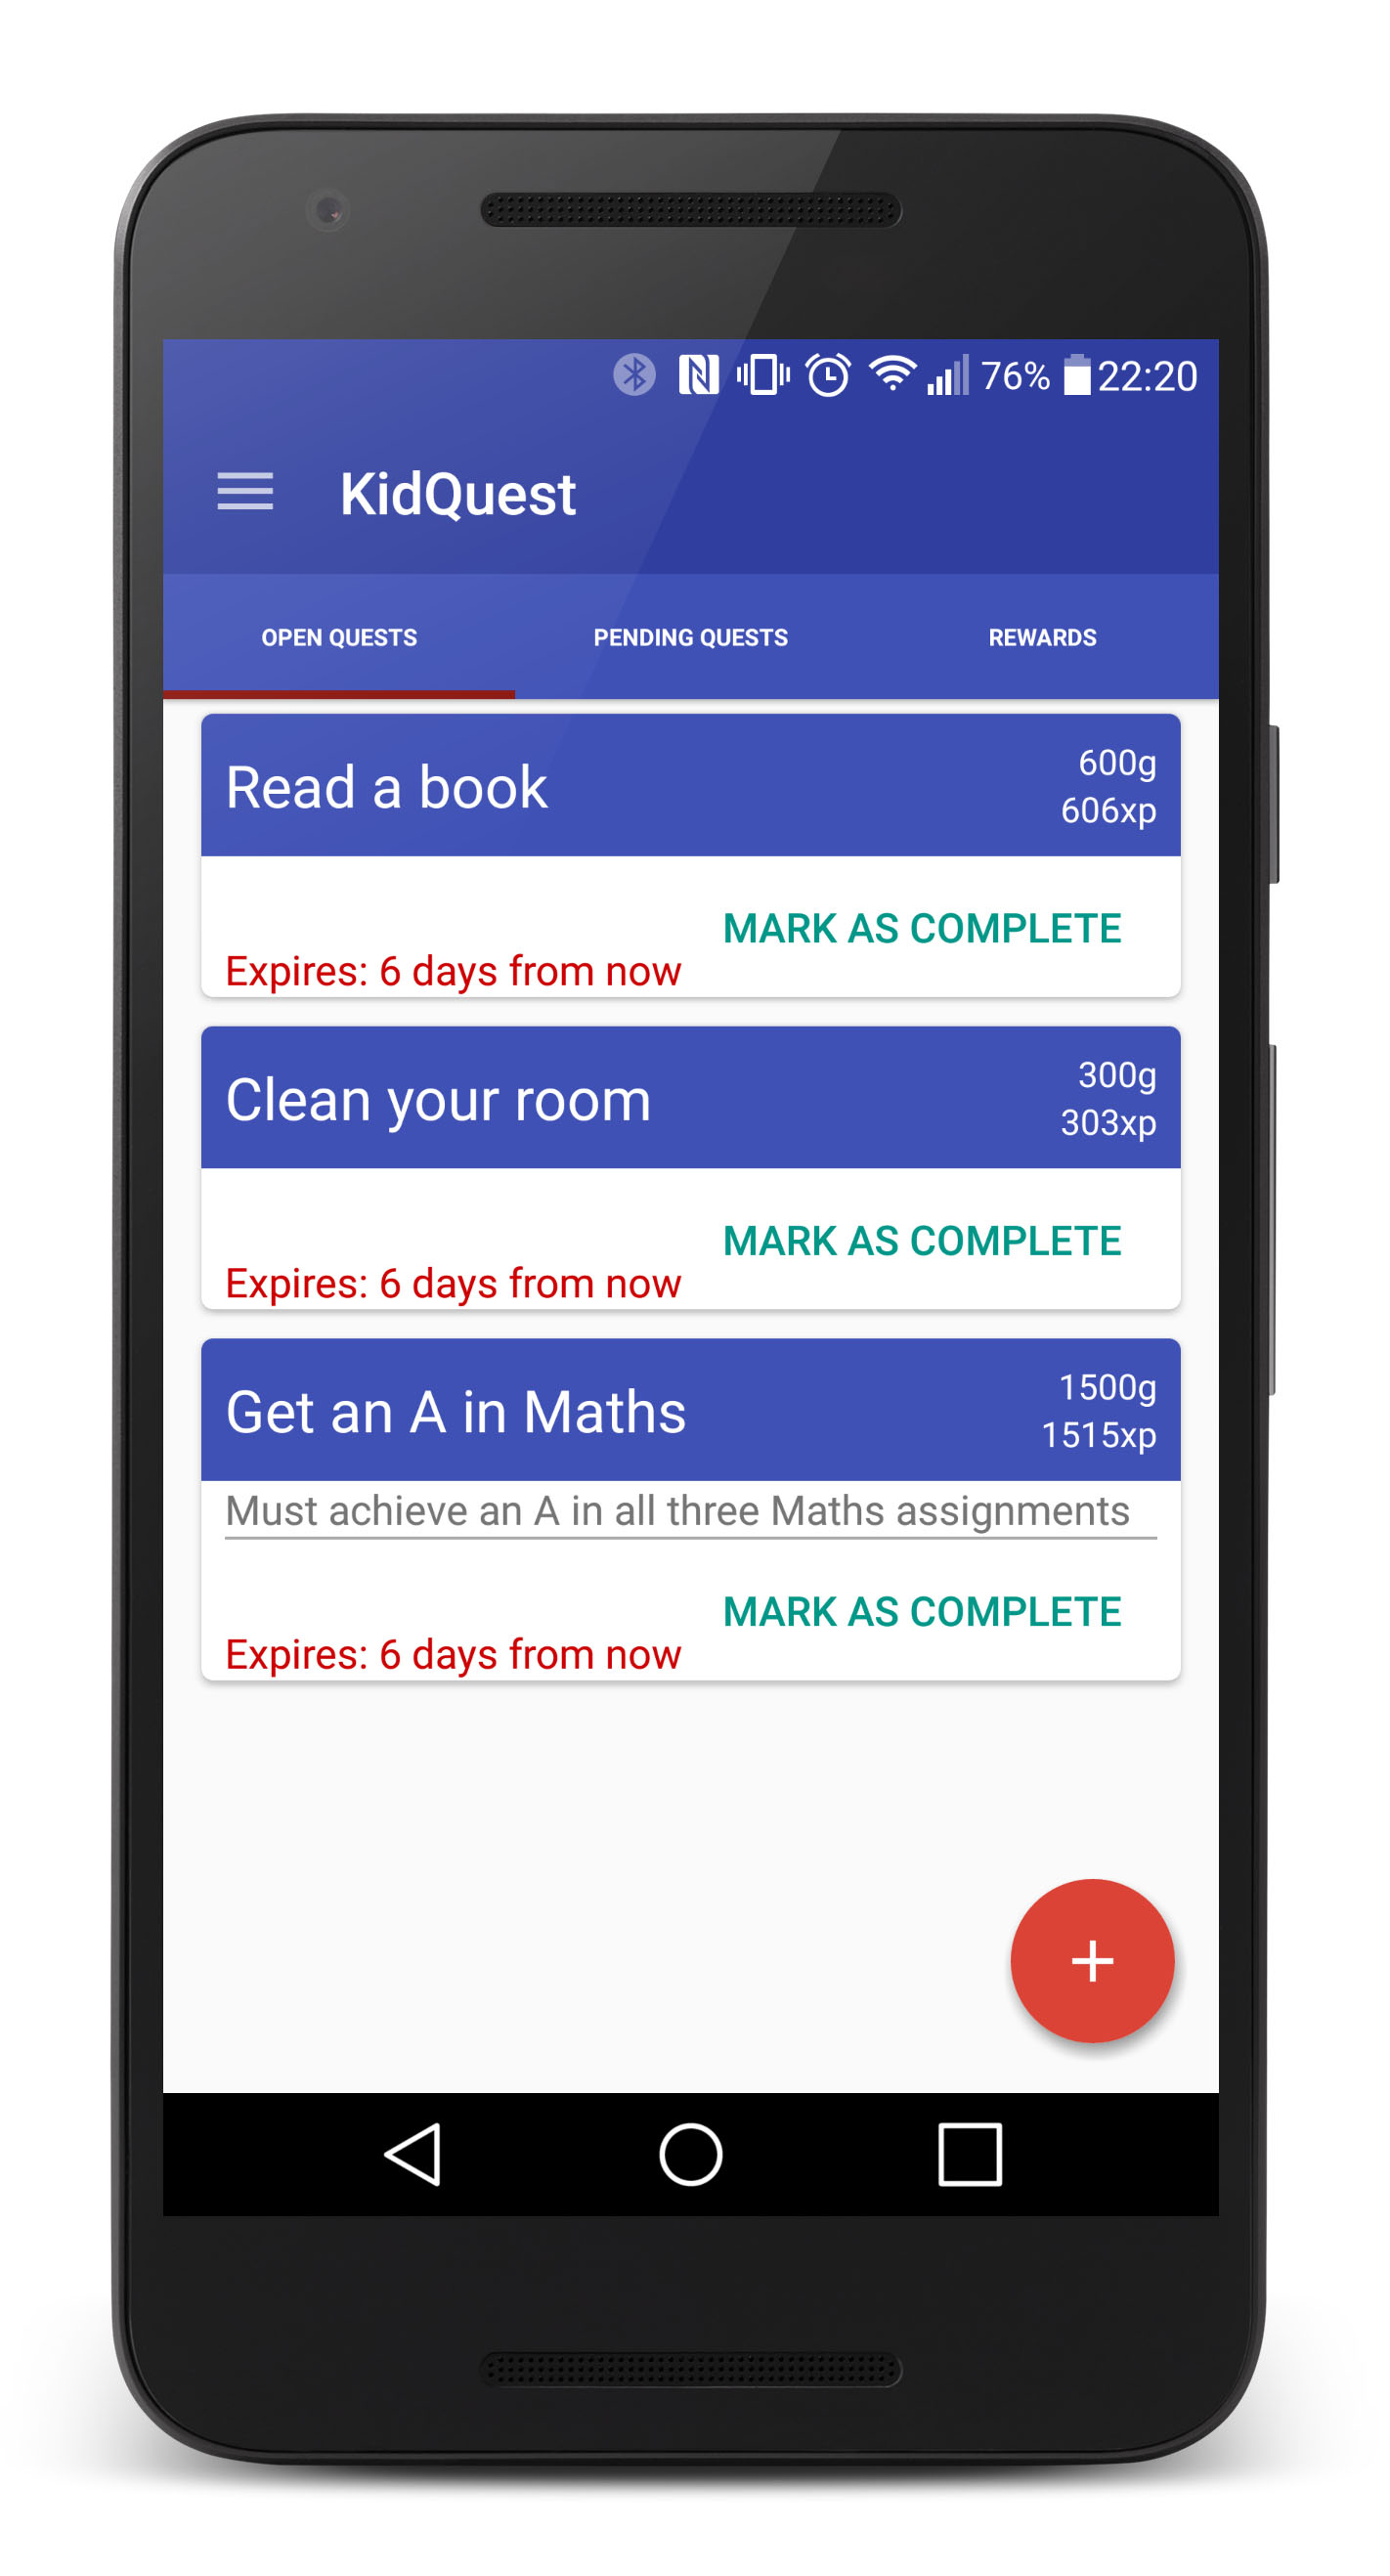
\includegraphics[width=1\linewidth]{../images/Screenshot/YourQuestsScreen.jpg} 
    \vspace{2ex}
  \end{minipage}%%
  \begin{minipage}[b]{0.25\linewidth}
    \centering
    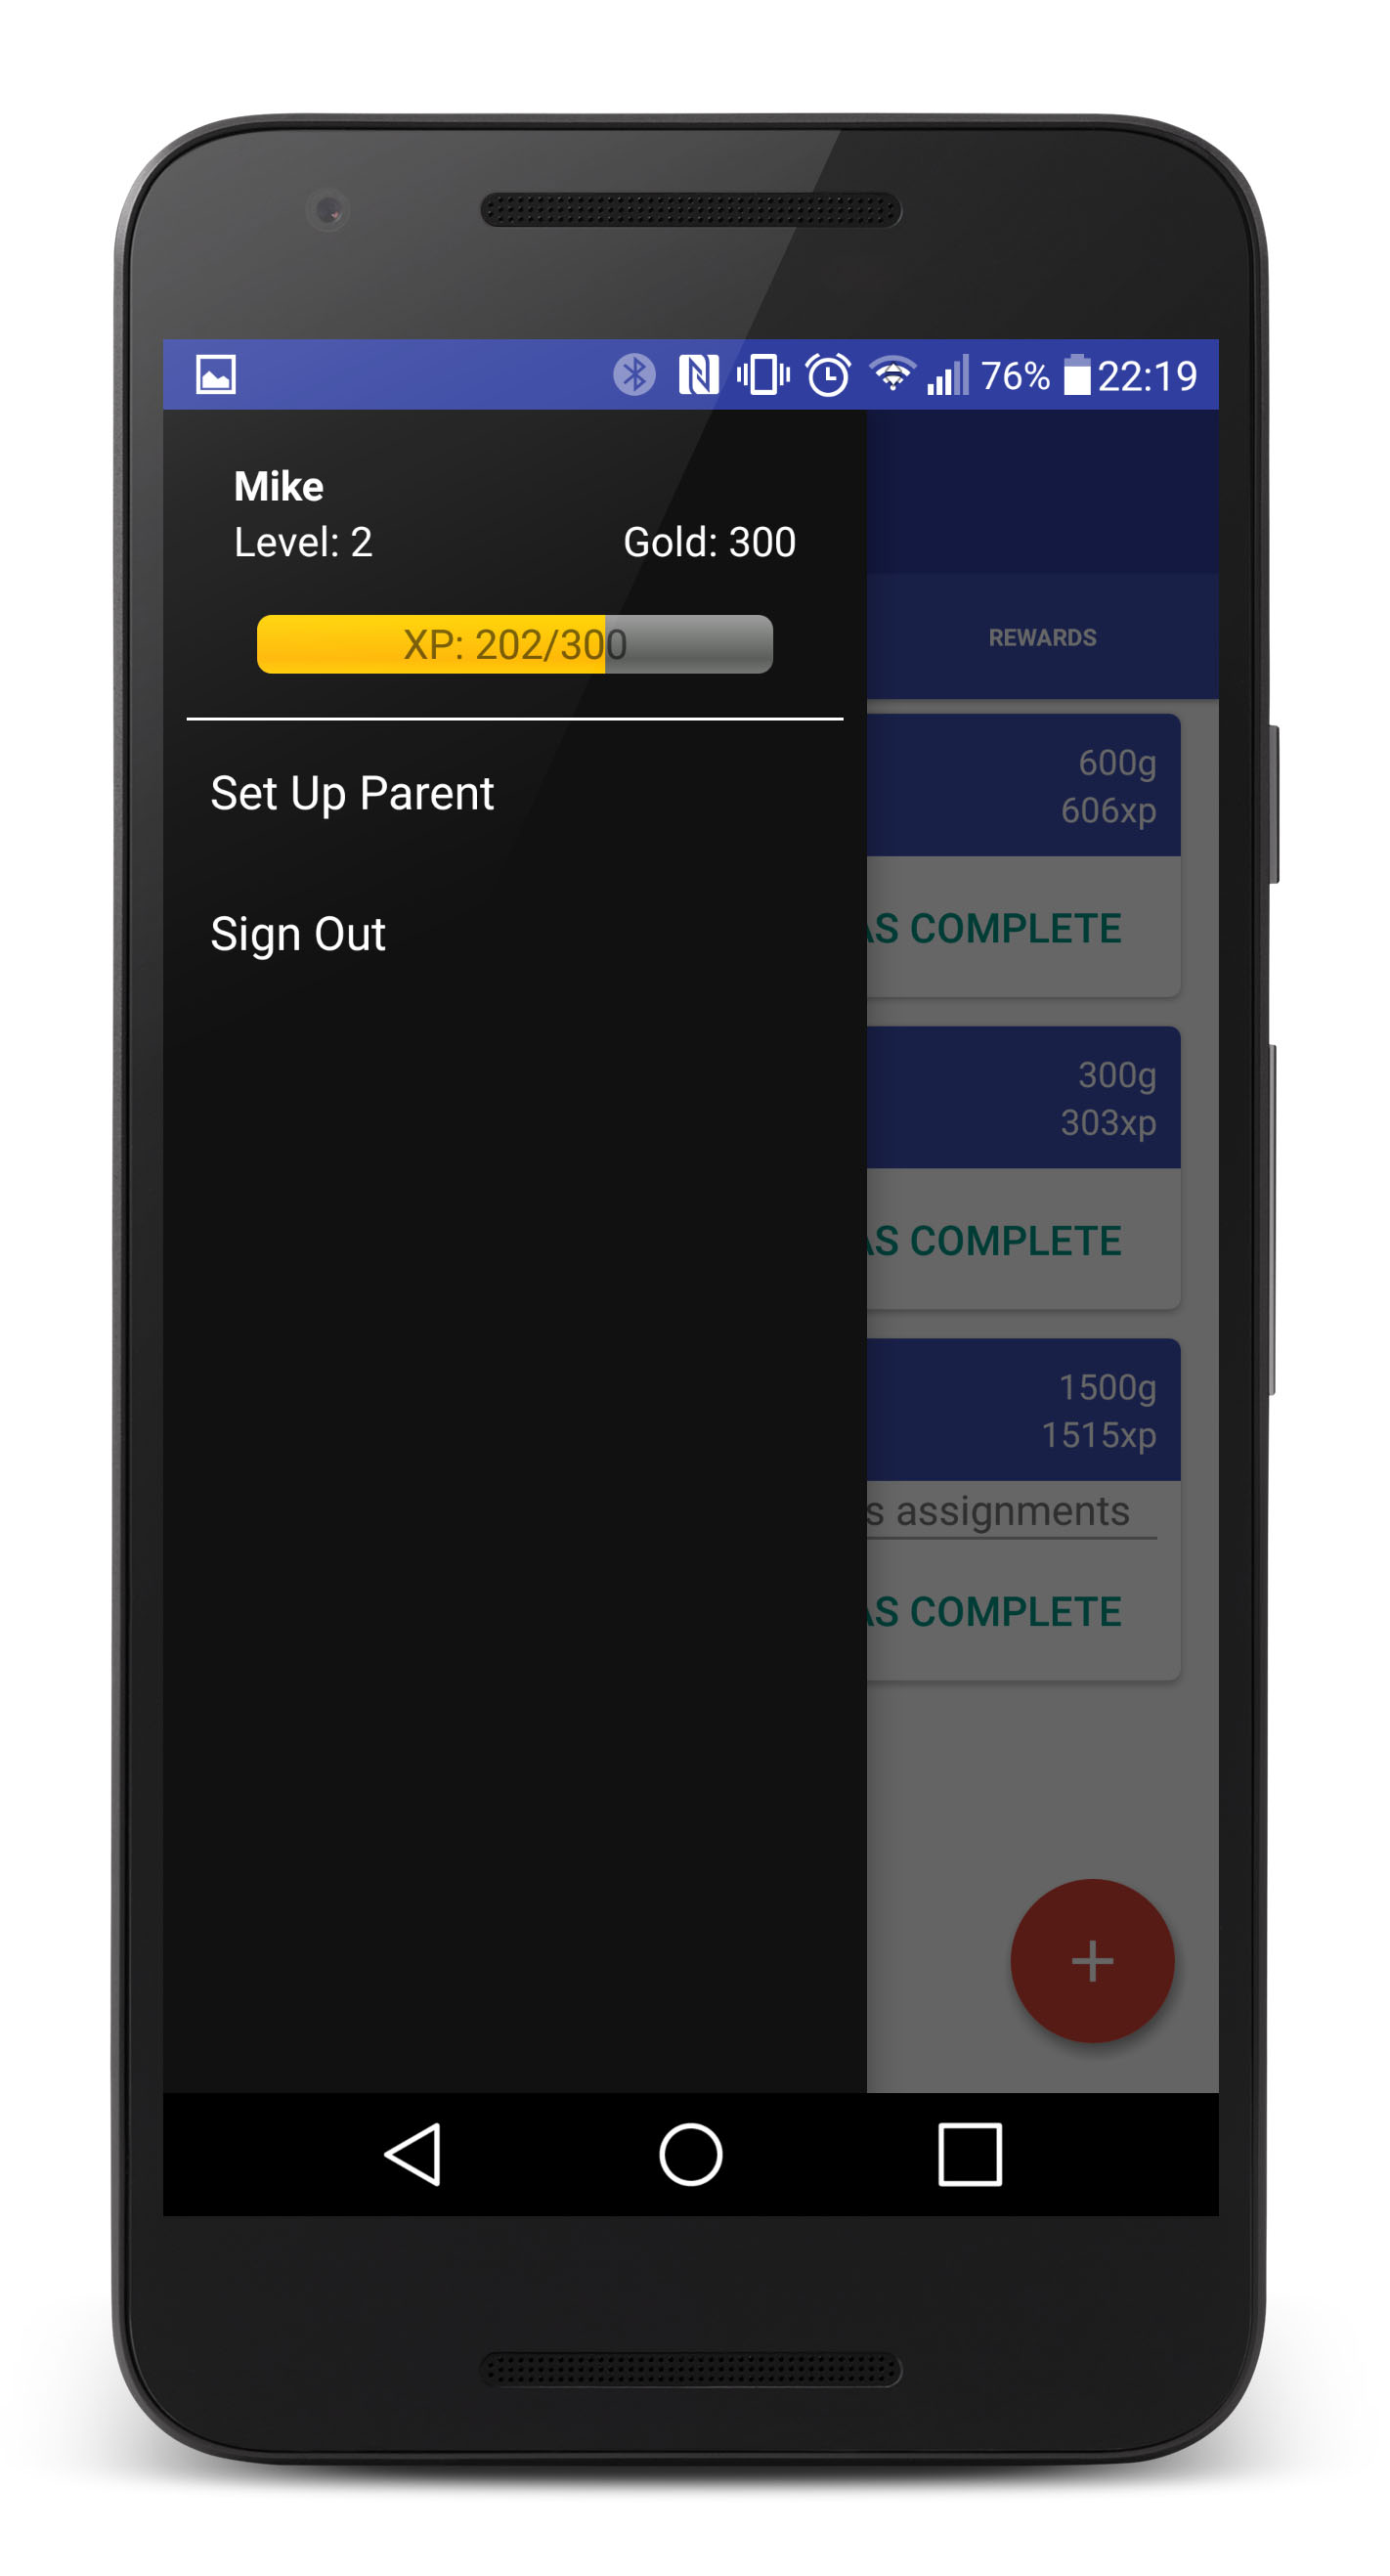
\includegraphics[width=1\linewidth]{../images/Screenshot/NavigationBar.jpg}
    \vspace{2ex}
  \end{minipage} 
  \begin{minipage}[b]{0.25\linewidth}
    \centering
    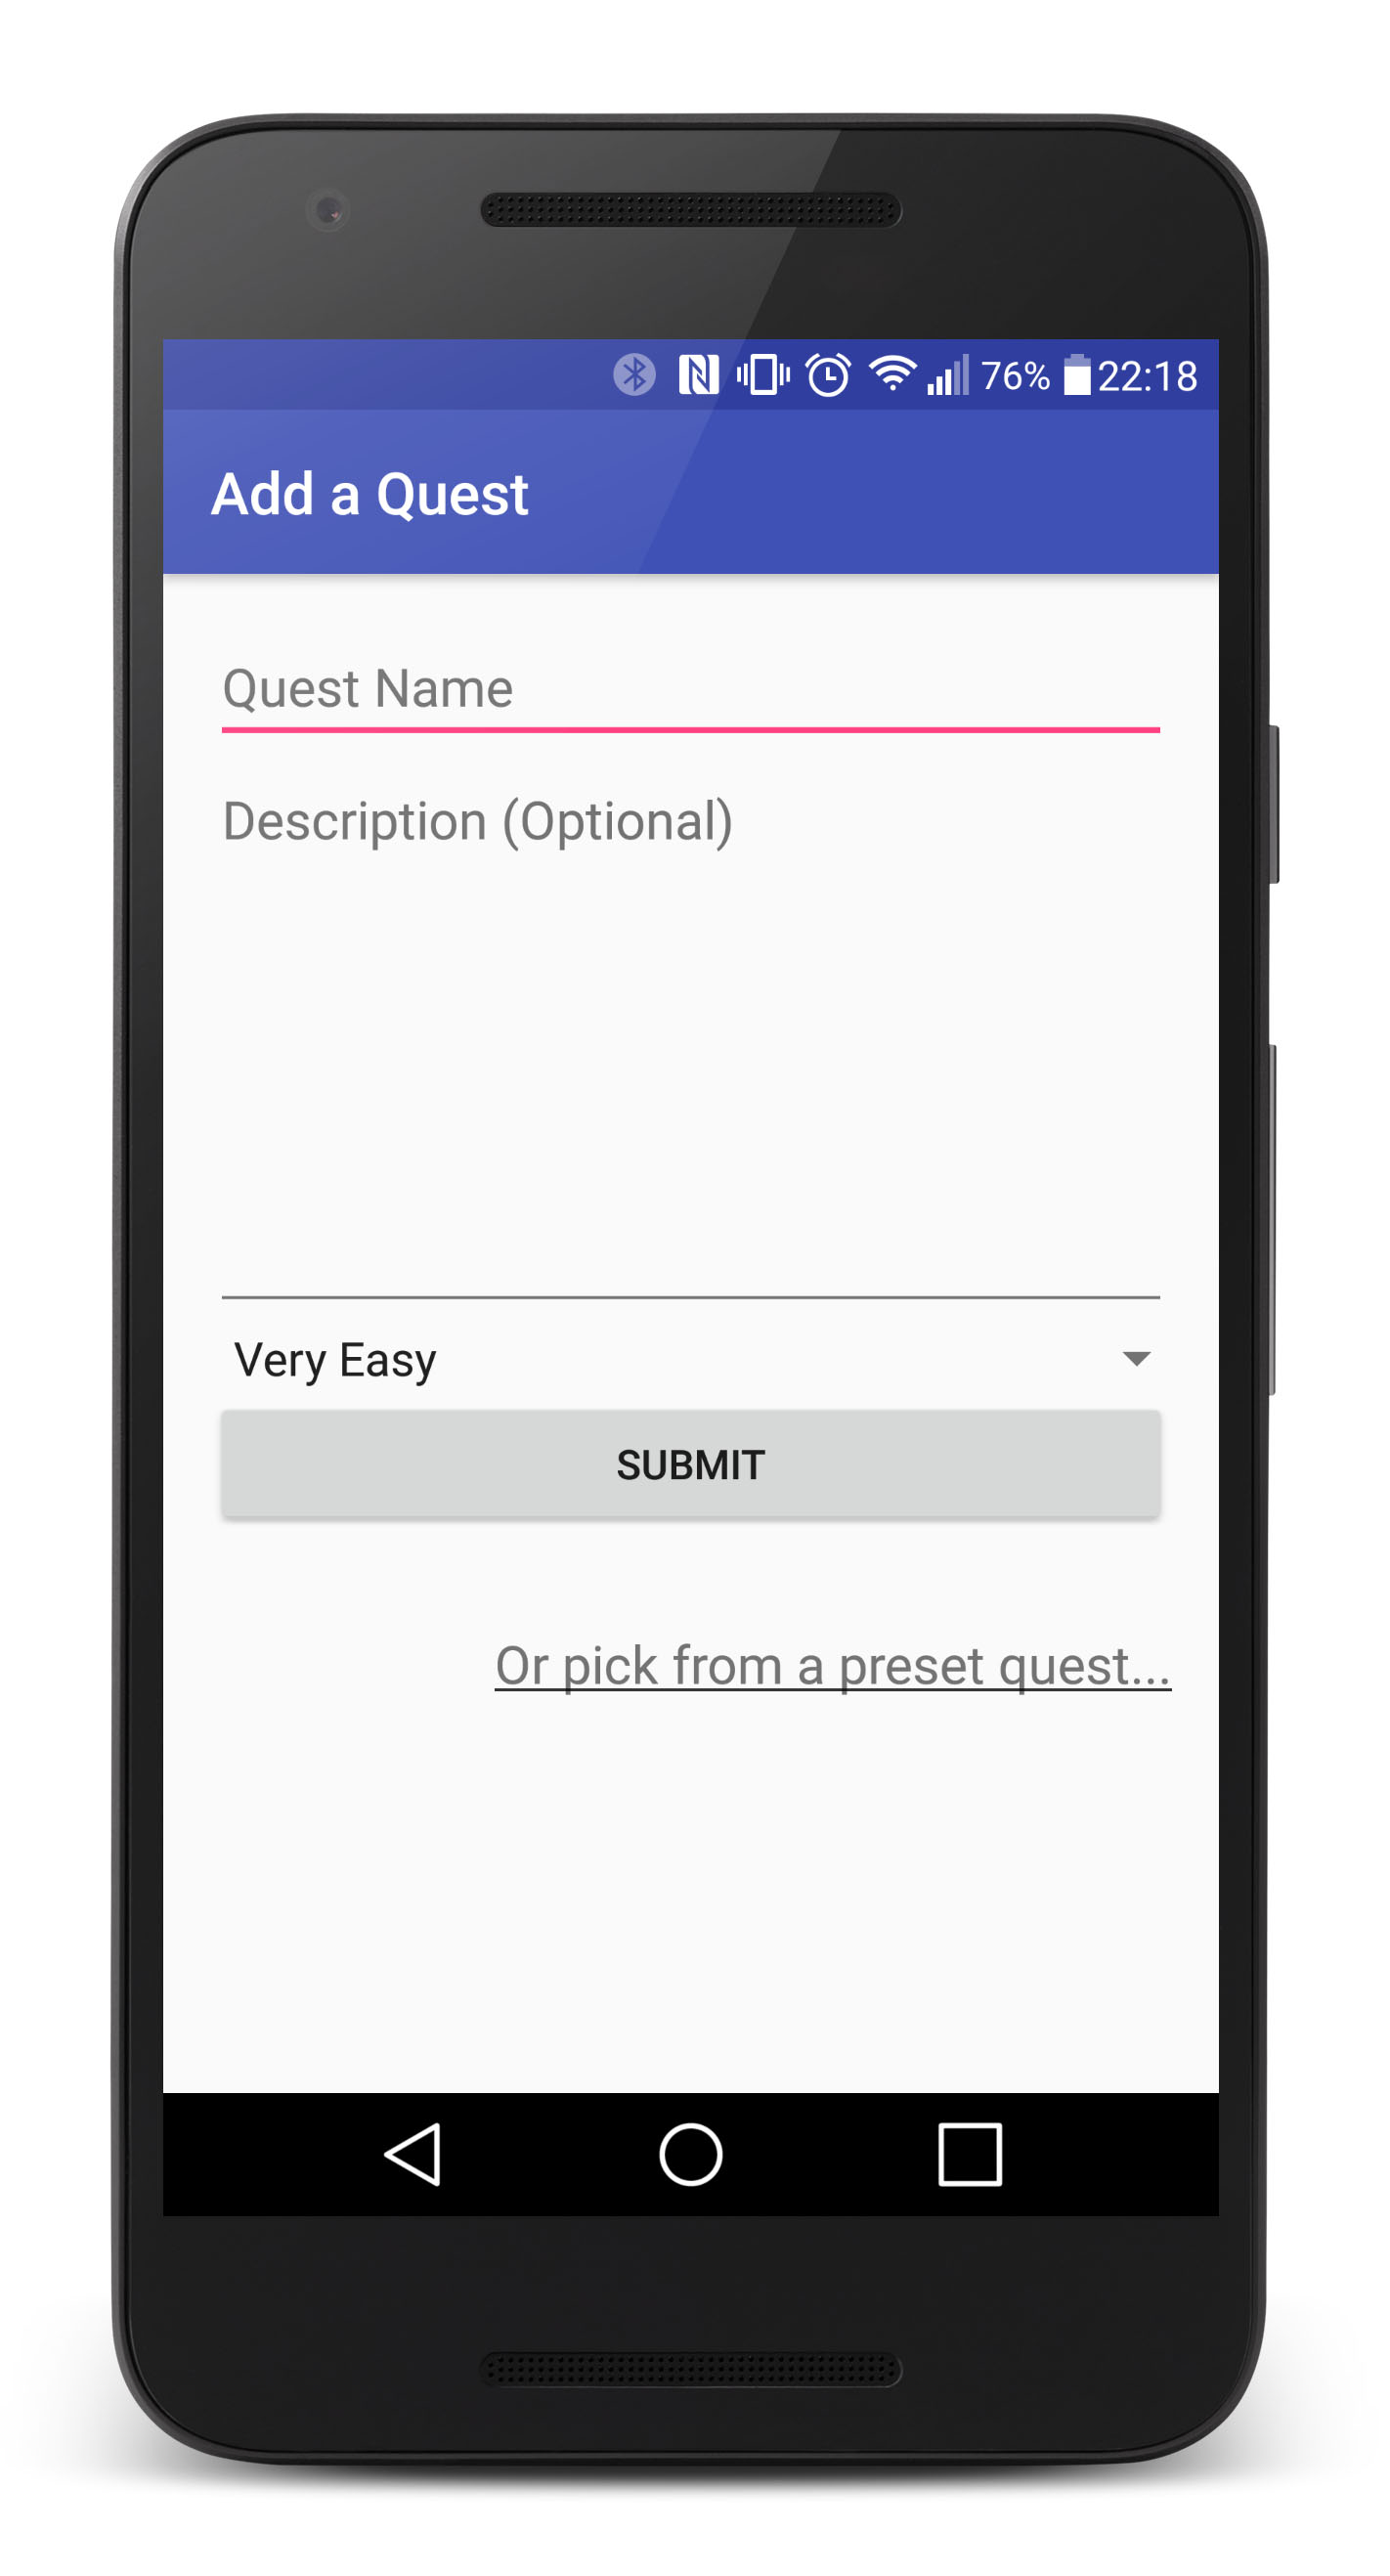
\includegraphics[width=1\linewidth]{../images/Screenshot/AddQuestScreen.jpg}
    \vspace{2ex}
  \end{minipage}%% 
  \begin{minipage}[b]{0.25\linewidth}
    \centering
    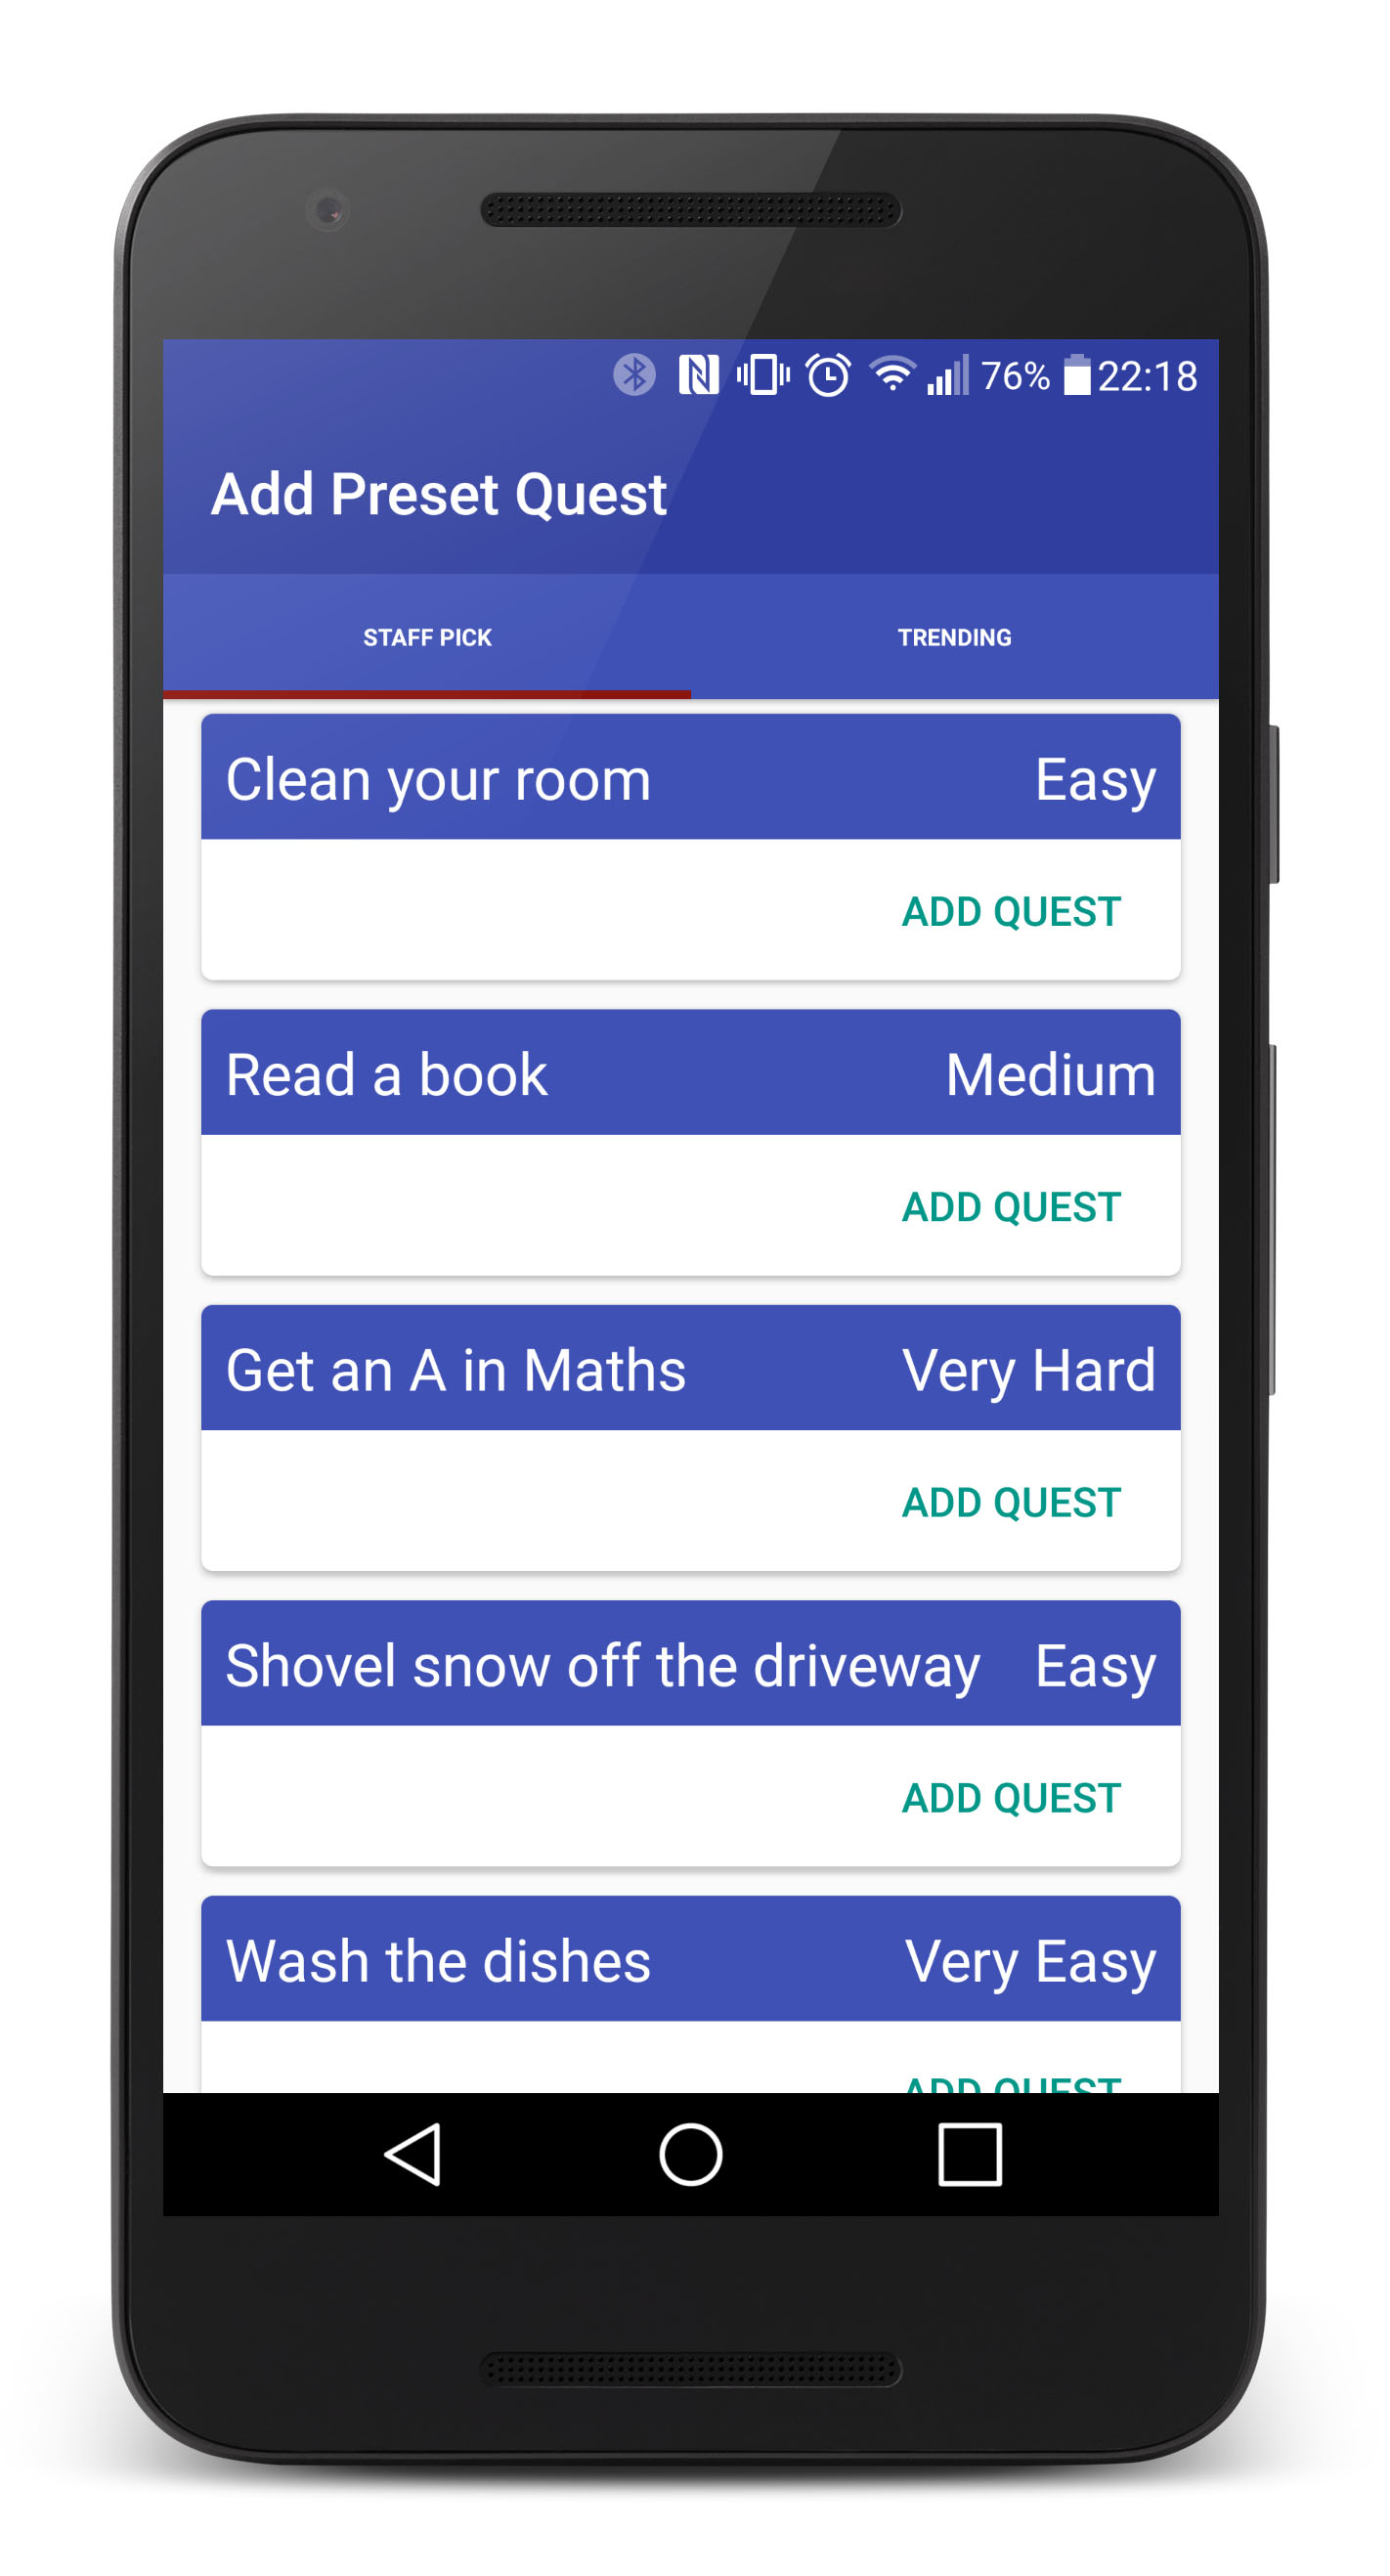
\includegraphics[width=1\linewidth]{../images/Screenshot/AddPresetQuestScreen.jpg}
    \vspace{2ex}
  \end{minipage} 
  \caption{Screenshots of the Project Artefact}
  \label{fig:screenshots}
\end{figure}

\section{Game Design}
\subsection{Rewards}
The rate at which these rewards are earned must be examined to ensure they still feel rewarding throughout. 
For example, if a quest returns 100 XP points and you require 300 XP to level up from level 1 to 2, this only requires you to complete three quests to level up, meaning these three quests feel rewarding as each quest is offering 1/3rd of a level.
However, if quests still offer 100 XP and you require 6000 XP to level from 30 to 31, the reward from the same quest is now worth 1/60th of what it was before, despite being the same difficulty to the user.
Therefore, some scaling of the rewards is required in the app to allow XP rewards to scale suitably with the XP required to level.
This scaling is referred to as `increasing cost' \citep{1_anderson_2016}.
Anderson also shows that it is important to determine reasonable caps for numerical relationships in video-games, to stop the increasing cost becoming out of proportion.

Anderson proposes that a useful pattern for these kinds of relationships is a classic triangular pattern, in which the first level requires 1 XP to level up, the second level requires 3 XP, the third requires 6 etc. To allow for more meaningful numbers to the user, I have multiplied the results of this formula by 100. The formula for this is $T_n= \frac{n(n+1)}{2} \times 100$, where $T$ is the XP required to level up and $n$ is the current level.

For XP rewards, the initial scaling formula involved using 60 XP as a base reward for a medium difficulty quest.
Then using the player's current level, it would derive a multiplier that would be used to scale the XP reward, using the following formula: 
$\textrm{XP Gained} = 60 \times \frac{(n - 1) \times k}{100} + 1$ where $n$ is the current character level and $k$ can be adjusted to determine the strength of the multiplier against the XP rewards.
Under this formula, if $k$ = 10, a character at level 31 would have a 3x multiplier on quests, meaning the same quest that gave them 60XP at level 1, now gives them 180XP.

However, when modelling this equation, the number of quests needed quickly becomes out of hand. 
At level 1, the player must complete 2 medium quests to level up - a reasonable starting point.
However by level 25 the player must complete 22 quests to level up and by level 100 the player must complete an extraordinary 84 medium difficulty quests.

Therefore, I also modelled triangular numbers for calculating the XP gained per quest. 
I adjusted the initial triangular numbers formula to $\textrm{XP Gained} = \frac{(n+2)(n+3)}{2} \times 10$ and found a suitable middle ground.
This formula gives the new user the feeling of progressing quickly, but the rate of quests per level quickly slows down to a limit of approximately 10 quests per level by level 100.
This will ensure that the player will still feel like they are progressing at a reasonable speed throughout.

The rate of quests required to level up using these two systems is mapped in figure \ref{fig:xprewardcomparison}.
This figure was mapped out assuming all quests completed were of medium difficulty, whereas in real usage the speed will increase or decrease depending on the difficulty of quests.

\begin{figure}
\centering
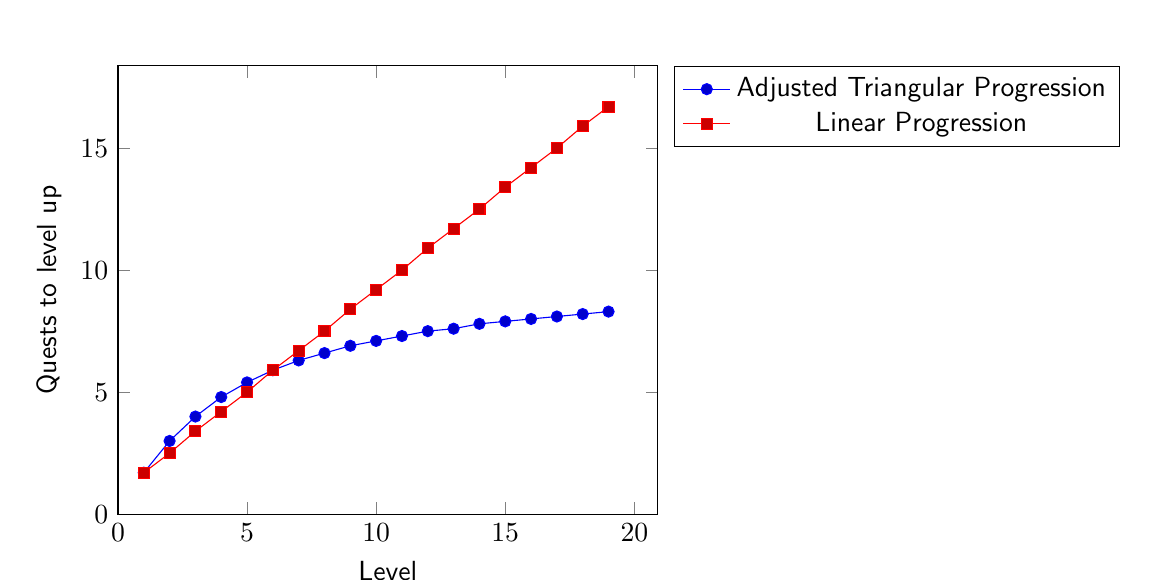
\begin{tikzpicture}
	\begin{axis}[
		xlabel=Level,
		ylabel=Quests to level up,
		xmin=0,
		ymin=0,
		legend pos = outer north east
	]
		\addplot coordinates {
			(1, 1.7)
			(2, 3)
			(3, 4)
			(4, 4.8)
			(5, 5.4)
			(6, 5.9)
			(7, 6.3)
			(8, 6.6)
			(9, 6.9)
			(10,7.1)
			(11,7.3)
			(12,7.5)
			(13,7.6)
			(14,7.8)
			(15,7.9)
			(16,8)
			(17,8.1)
			(18,8.2)
			(19,8.3)
		};
		\addlegendentry{Adjusted Triangular Progression}
		\addplot coordinates{
			(1, 1.7)
			(2, 2.5)
			(3, 3.4)
			(4, 4.2)
			(5, 5)
			(6, 5.9)
			(7, 6.7)
			(8, 7.5)
			(9, 8.4)
			(10, 9.2)
			(11, 10)
			(12, 10.9)
			(13, 11.7)
			(14, 12.5)
			(15, 13.4)
			(16, 14.2)
			(17, 15)
			(18, 15.9)
			(19, 16.7)
		};
		\addlegendentry{Linear Progression}
	\end{axis}
\end{tikzpicture}
\caption{A comparison of two XP reward systems}
\label{fig:xprewardcomparison}
\end{figure}

\subsection{Gold Rewards}
A key goal of the project is achieving long term motivation for children, and to avoid the non-continuous effects mentioned by \cite{deci2001extrinsic} in chapter 2 research.
In order to achieve this goal, I implemented two key elements to the rewards earned from a quest.

Firstly, in order to discourage Child users from delaying performing a task, I implemented a system that gradually diminishes the maximum achievable gold reward for a quest over time. 
In this system, a quest is added with an expiry date value, which defaults to one week from the quest creation date, unless otherwise specified.
At around halfway through the time available to complete the task, the reward from the quest will begin to reduce at a steady rate for the remaining time.
Eventually, if the task remains incomplete until the expiry date, the gold reward drops to zero, the quest expires and the quest is removed from their tasks.
This is an example of an `open loop system', where previous performance has no bearing on the current reward.

Secondly, I extended this system to base the given reward for a quest off of the Child's time-based performance in their last three quests.
This is referred to as a `closed loop system', where the reward amount is calculated based off previous rewards.
The end result is that if a Child allows a quest to begin expiring, it will effect the following three quests rather than just the current one.
This system encourages the user to maintain a streak of fulfilling tasks in a timely manner and discourages them from allowing a quest to expire as it will not just be that reward that is effected, but their rewards for the next three quests.
It is intended that this will influence children to begin thinking about their tasks in a long-term manner.
If the user has completed fewer than three quests, the effect is ignored as there is not enough data.
The reward is calculated using the following equation: $y_k = ax_k + by_{k-1} + cy_{k-2} + dy_{k-3}$ where $k$ is the quest, $y$ is the reward for that quest and $a$-$d$ are adjustable coefficients that sum up to 1.
 
A comparison of the two types of rewards can be seen in figure \ref{fig:rewardcomparison}.

\begin{figure}[ht]
\centering
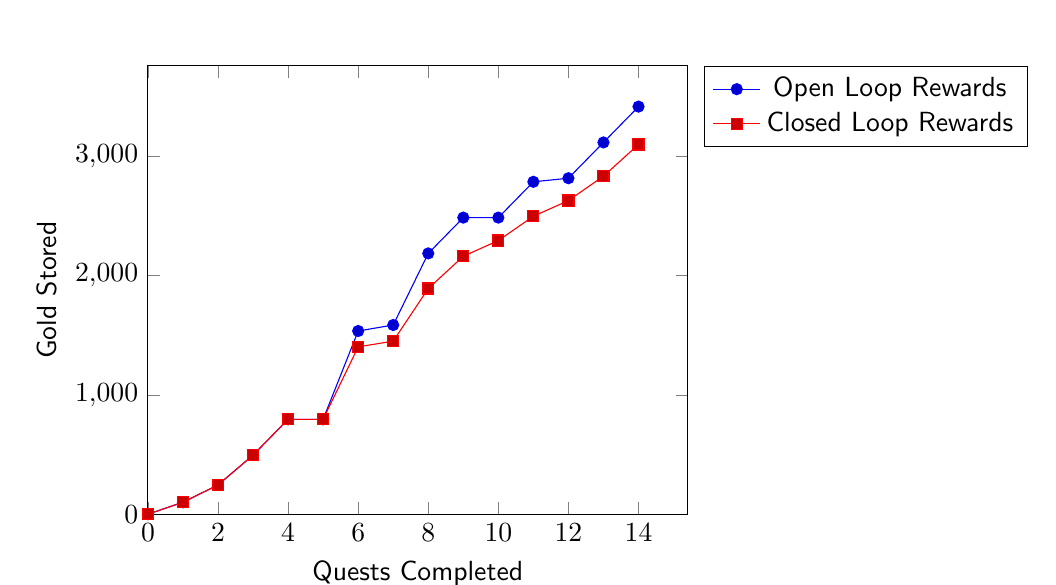
\begin{tikzpicture}
	\begin{axis}[
	xlabel=Quests Completed,
	ylabel=Gold Stored,
	ymin=0,
	xmin=0,
	legend pos = outer north east
	]
		\addplot coordinates{
			(0,0)
			(1,100)
			(2,245)
			(3,495)
			(4,795)
			(5,795)
			(6,1535)
			(7,1585)
			(8,2185)
			(9,2485)
			(10,2485)
			(11,2785)
			(12,2815)
			(13,3115)
			(14,3415)
		};
		\addlegendentry{Open Loop Rewards}
		\addplot coordinates{
			(0,0)
			(1,100)
			(2,245)
			(3,495)
			(4,795)
			(5,795)
			(6,1402)
			(7,1450)
			(8,1891)
			(9,2161)
			(10,2293)
			(11,2496)
			(12,2628)
			(13,2832)
			(14,3098)
		};
		\addlegendentry{Closed Loop Rewards}
	\end{axis}
\end{tikzpicture}
\caption{A comparison of the two reward types}
\label{fig:rewardcomparison}
\end{figure}

\subsection{Evaluation}
In my evaluation of the artefact, I found that the triangular XP system provided a much more rewarding feel to the user. 
The application still provided a very fast gain when the user first starts using the app, but quickly levels off to a reasonable amount.
The linear system quickly spiralled, which I felt was counter-intuitive to the intended motivational effects and would ultimately dishearten users who would have otherwise enjoyed the app.

The gold and XP reward systems follow two separate paths.
Where both the XP gained per quest and the XP required to level up increase each level, the gold rewards remain at a continuous gain and do not involve player levels.
With XP, I preferred the system that rewards the player with more XP, whereas with gold rewards, the system that provided less was preferred.
This is mainly due to the inclusion of a reward shop in the project, which exchanges some of the Child's gold storage for a real life reward set by the Parent. 
Therefore, in order for this to work successfully, the amount of gold that a child earns must remain stable.

\section{Testing}
Unfortunately, when developing a REST API, it is difficult to manually write and send the request to the API to test it.
Programs and scripts exist to ease the process somewhat, but I found the easiest way to be automating the requests entirely. 
As a main principle of REST is to plan out the specific endpoints that can be messaged, it becomes rather simple to deduce automated tests by sending examples of valid and invalid requests to endpoints and then verifying the stored data.
For example, the endpoint of `/api/users/$userId$/' allows two request types, GET and PUT, which easily generates four test cases.
\begin{itemize}
	\item{Valid GET}
	\item{Invalid GET}
	\item{Valid PUT}
	\item{Invalid PUT}
\end{itemize}  
%TODO: Research what test generation this is

However, this raises issues when considering that a request could be invalid for multiple reasons, and simply testing for invalid/valid may not reach adequate code coverage.
A PUT request, for example, could be invalid due to an email address already existing in the system, or no new data being entered about the user. Both of these reasons are in separate sections of the code that each require their own tests.
This issue is highlighted by \cite{4597151}, who states that testing a program tells us `little about its quality', arguing that the quality of a test case far outweighs sheer quantity of tests.
Because of this, it must be analysed whether or not the test cases achieve sufficient code coverage, rather than just relying on the entry points into the software.
Luckily, the python package `coverage.py' allows for simple analysis of unit tests to determine the current code coverage for tests, which will provide a higher rate of confidence.

\subsection{Test-Driven Development and Unit Testing}
In the creation of a REST API, it is much easier to develop a test plan due to the clearly laid out workflow of the user. 
From the server's point of view, there are only a handful of requests that a user can make, and a small number of tests for those requests. 
Before writing each endpoint of the server, I developed a unit test  that would test the various inputs to this endpoint.
Usually, these unit tests consisted of python code to create and send a request to the testing server and then check the database to verify if the data was stored correctly.

I used an extension library of Flask called Flask-Testing, which streamlined the process of writing and running unit tests.
The library allows you to create a new instance of your Flask application with a separate configuration file which can be changed to make the app connect to a different MySQL database file - in this case it connected to a freshly generated and empty test database.
Then, as each separate test case is run, I used the library to delete the test database and regenerate it to ensure that previous unit tests would not interfere with new tests.

For example, the following code is a simple test that creates a Child user on the server, then attempts to get the user details from the server without authorising itself first. 
The test will pass if the server correctly rejects the request with a `401: Not Authorised' error or fail otherwise.
\lstinputlisting[language=python]{codesnippets/serverunittest.py}

\subsection{Integration Testing}
Integration testing encompasses tests that ensure the various parts of the project work together correctly.
For example, in this project, integration tests would test that the server and mobile app are able to correctly function together, by ensuring that the app can correctly send requests and that the server receives those requests as they were sent.

As the large majority of functionality took place in the server application, much of the integration testing that took place was to test that the mobile application was correctly requesting, sending and displaying data that it received from the server.

\subsection{Black Box Testing}
Black box testing describes the testing of software without using explicit knowledge of the code.
Essentially, it is testing by using that the usage of the application is correct.
The android application was mostly tested using black box testing by listing out various actions that a user may perform on the app - whether valid or invalid actions - and testing that they are correctly accepted or rejected.

Due to the nature of the server code being primarily machine-to-machine communication, I consider black box testing to be inappropriate for testing the server.

\subsection{White Box Testing}
White box testing is the testing of a system using the knowledge of how the code works and encompasses tests such as boundary testing and equivalence partitioning testing.
This was mostly performed on the server side code due to the fact that the majority of the android code was GUI based and provided no actual functionality.

\subsection{Regression Testing}
Regression testing is the practice of retesting the previously tested parts of the software to ensure that they are still performing correctly after a change elsewhere in the code, it can also be used to describe the process of testing previously detected and fixed bugs to determine that they have not reappeared.

This was made significantly easier by the implementation of strong automated unit tests, which allowed me to quickly retest the majority of the code by rerunning the test suite.
I also followed a common development practice where a unit test is added for each defect found within the code to detect the presence of that bug specifically. 
This allowed me to easily spot any recurrences of legacy bugs that would have otherwise gone unnoticed.

\section{Problems Encountered}
\subsubsection{Server Rewrite}
As previously mentioned, issues arose regarding my assumptions about the GCM service.
Initially, it was planned to have most of the functionality within the phone application and have monitoring phones communicate with it.
Due to this, initial prototypes of both server and applications were inappropriate for the development of the system and had to be reworked.
This incurred large delays in the progress of the artefact as alternative technologies were considered altogether.
It was debated whether Flask was still suitable for the task, as I believed that all the extra code needed in the server might become too messy when written for Flask.

There were also initial issues with implementing automated testing within Flask, as I had not understood the extra requirements needed to run a separate, debugable instance of Flask and as such struggled to implement unit tests that successfully tested the web services.
However, with the discovery of both the Flask-Testing library and the GCM library it was found that the Flask code that had already been written would be able to reworked into a suitable API.

\subsubsection{Data Loss}
As predicted in the risk analysis in chapter 1, there was a small issue with data loss during the development of the application.
During a regular reformat of my PC's hard drive, a small amount of code on the machine that had not been saved in a remote location was irretrievably deleted.
However, by following the plans set out in the risk analysis, this issue was greatly mitigated by the fact that I had regularly committed and pushed code to the git repository. 
The lost code was not able to be recovered, but the loss was kept to an absolute minimum as the last commit had taken place only a few hours before the reformat.


%500-1000 words
%!TEX root = ../main.tex
\chapter{Conclusion}

Lorem ipsum dolor sit amet, consectetur adipisicing elit, sed do eiusmod tempor incididunt ut labore et dolore magna aliqua. 
Ut enim ad minim veniam, quis nostrud exercitation ullamco laboris nisi ut aliquip ex ea commodo consequat. 
Duis aute irure dolor in reprehenderit in voluptate velit esse cillum dolore eu fugiat nulla pariatur. 
Excepteur sint occaecat cupidatat non proident, sunt in culpa qui officia deserunt mollit anim id est laborum.


%TC:ignore

%\nocite{*} %Take this out if you don't want it to show all the references and only the ones you've referenced 
%30-50 references traditionally.
\bibliography{references}

%!TEX root = ../main.tex
\begin{appendices}

\chapter{Sheldon Book Grading Structure}

\chapter{Wireframe Designs}
\label{appendix:wireframes}

\begin{figure}[ht] 
  \label{ fig7} 
  \begin{minipage}[b]{0.5\linewidth}
    \centering
    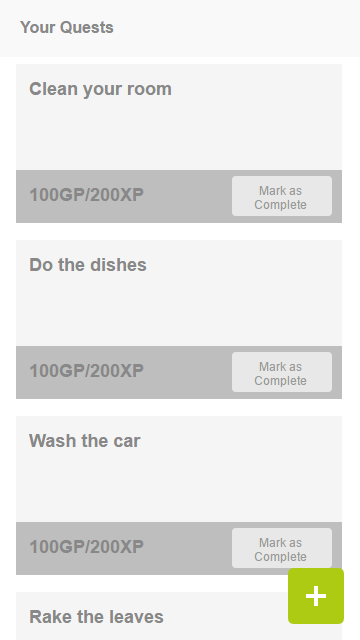
\includegraphics[width=.5\linewidth, frame]{../images/Wireframes/YourQuestsScreen.png} 
    \caption{Your Quests Screen} 
    \vspace{4ex}
  \end{minipage}%%
  \begin{minipage}[b]{0.5\linewidth}
    \centering
    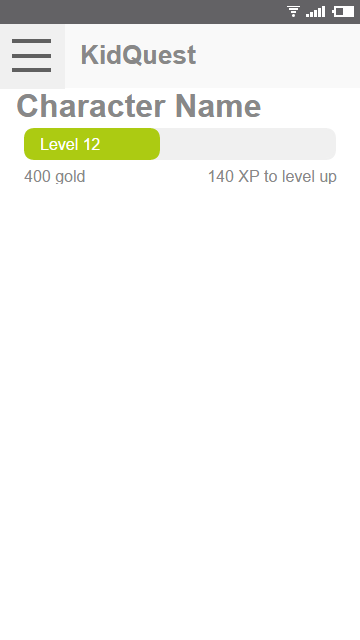
\includegraphics[width=.5\linewidth, frame]{../images/Wireframes/MainScreen.png}
    \caption{Landing Page} 
    \vspace{4ex}
  \end{minipage} 
  \begin{minipage}[b]{0.5\linewidth}
    \centering
    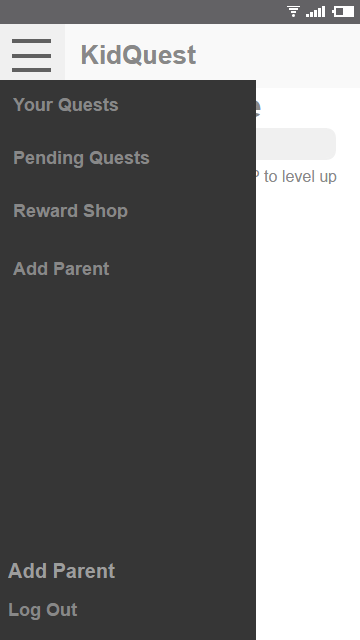
\includegraphics[width=.5\linewidth, frame]{../images/Wireframes/NavigationScreen.png}
    \caption{Navigation Sidebar} 
    \vspace{4ex}
  \end{minipage}%% 
  \begin{minipage}[b]{0.5\linewidth}
    \centering
    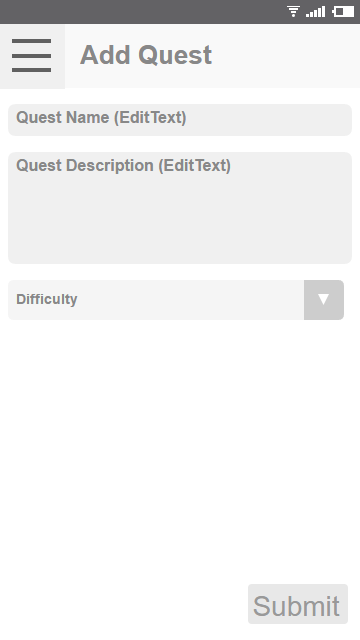
\includegraphics[width=.5\linewidth, frame]{../images/Wireframes/AddQuestScreen.png}
    \caption{Add Quest Form} 
    \vspace{4ex}
  \end{minipage} 
  \caption{Wireframe Designs for the KidQuest Application}
\end{figure}

%!TEX root = ../main.tex
\chapter{Notifications}
\label{appendix:pushnotifications}

\begin{tabular}{|c|c|}
	\hline
	\textbf{Event} & \textbf{Notifcation Text} \\
  	\hline
  	Quest Complete & ``You have completed a quest!'' \\
  	\hline
  	Quest Confirmed & ``A child you are monitoring has finished a task and requires approval'' \\
  	\hline
  	Quest Added & ``A new quest is available!'' \\
  	\hline
  	Level Up & ``You have levelled up!'' \\
  	\hline
  	Reward Added & ``New rewards are available in the store!'' \\
  	\hline 
  	Reward Purchased & ``A child you are monitoring has purchased a reward from the store'' \\
  	\hline
\end{tabular}

\end{appendices}

%TC:endignore

\end{document}